\documentclass[a4paper, 12pt]{article}

\usepackage{a4wide}
\usepackage[utf8]{inputenc}
\usepackage[russian]{babel}
\usepackage[pdftex]{graphicx}
\usepackage{amsmath}
\usepackage{amssymb}
\usepackage{amsfonts}
\usepackage{graphicx}
\usepackage{hyperref}
\usepackage{verbatim}
\usepackage{indentfirst}
%\usepackage{listings}
\usepackage{alltt}
\setlength{\parindent}{1.25cm}

\newtheorem{myComment}{Замечание}
\newtheorem{myDef}{Определение}
\newtheorem{myProp}{Свойство}
\newtheorem{myTeor}{Теорема}
\newcommand{\dbtilde}[1]{\accentset{\approx}{#1}}
\DeclareMathOperator{\sign}{sign}

\begin{document}

\thispagestyle{empty}

\begin{center}
\vspace{-3cm}

\includegraphics[width=0.5\textwidth]{msu.png}\\
{\scshape Московский государственный университет имени}\\
М. В. Ломоносова\\
Факультет вычислительной математики и кибернетики\\
Кафедра системного анализа

\vfill

{\LARGE Отчёт по практикуму}

\vspace{1cm}

{\Huge\bfseries <<Суперкомпьютеры и параллельная обработка данных>>}\\
{\LARGE Параллельная реализация алгоритма быстрой сортировки}
\end{center}

\vspace{1cm}

\begin{flushright}
  \large
  \textit{Студент 415 группы}\\
  А.\,Н.~Ашабоков

  \vspace{5mm}


\end{flushright}

\vfill

\begin{center}
Москва, 2019
\end{center}

\newpage
\setcounter{tocdepth}{1}
\tableofcontents

\newpage
\normalsize

\section{Обоснование выбора алгоритма для параллельной реализации}
Алгоритмы сортировки являются одними из наиболее важных и часто используемых алгоритмов при написании программ, связанных с обработкой больших массивов данных, а алгоритм быстрой сортировки является наиболее эффективным и распространенным.

\section{Ссылка на описание выбранного математического алгоритма в энциклопедии AlgoWiki}
Описание выбранного алгоритма можно найти по ссылке: 

algowiki-project.org/ru/Участник:Ashabokov\_415/Алгоритм\_быстрой\_сортировки 


\section{Результаты запусков на суперкомпьютере Ломоносов}
Для оценки эффективности и масштабируемости программы были проведены серии испытаний с различными конфигурациями. Для каждой конфигурации $(N, P)$, где $N$ --- длина входного массива, $P$ --- число задействованных процессоров, было произведено по $3$ запуска программы, после чего производилось усреднение полученных для фиксированной конфигурации результатов. В качестве входных данных были взяты случайным образом сгенерированные массивы длины $[500 : 2300]$ с шагом $200$, значения количества задействованных процессоров были взяты из диапазона $[8, 128]$ с шагом $8$. Результаты испытаний приведены в таблице:

\begin{center}
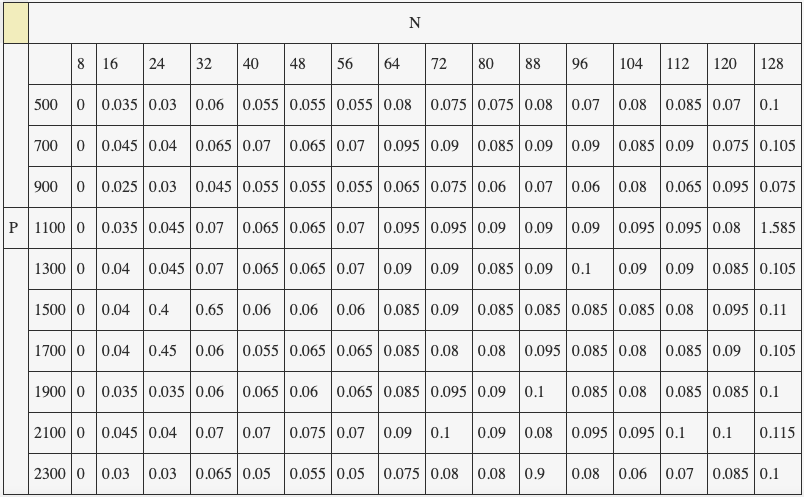
\includegraphics[width=0.8\textwidth]{tab_1.png}\\
Таблица 1: Время выполнения программы для различных конфигураций. 
\end{center}

\section{График сильной масштабируемости с пояснениями}
Для начала введем необходимые термины.

\begin{myDef}
Сильная масштабируемость (strong scaling) - зависимость производительности $R$ от количества процессоров $p$ при фиксированной вычислительной сложности задачи $(W=const)$.
\end{myDef}
\begin{myDef}
Производительность (performance) $R=Op/t$ определяется количеством операций $Op$, производимых данным компьютером в единицу времени.
\end{myDef}
\begin{myDef}
Вычислительная сложность (computational complexity) задачи $W$ - количество основных вычислительных шагов лучшего последовательного алгоритма, необходимых для решения задачи на одном процессоре.
 \end{myDef}
 
\begin{center}
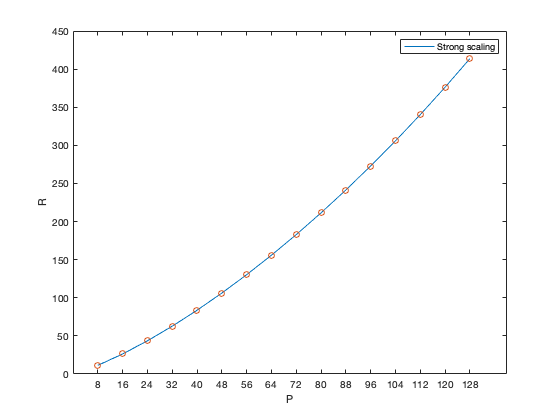
\includegraphics[width=0.8\textwidth]{str_sc.png}\\
Рис. 1: График сильной масштабируемости. \label{pic_1}
\end{center}
Из приведенного выше графика видно, что с ростом количества процессоров  $P$ происходит рост производительности $R$ при фиксированном значении вычислительной сложности задачи $W$.

\section{Объяснение полученных результатов}
На \hyperref[pic_1]{Рис.1} и приведенных в \href{https://algowiki-project.org/ru/Участник:Ashabokov\_415/Алгоритм\_быстрой\_сортировки}{статье} \hyperref[stat_1]{[2]} графиках можно наблюдать рост производительности при увеличении числа процессоров. Относительно быстрый рост производительности, наблюдаемый на \hyperref[pic_1]{Рис.1} можно объяснить тем, что при увеличении числа процессоров происходит сильное сокращение числа сортируемых на каждом из процессоров данных. Из приведенных в \hyperref[stat_1]{[2]} рассуждений следует, что данный алгоритм имеет относительно хорошую положительную масштабируемость по числу процессоров и отрицательную масштабируемость по числу входных данных. Правда, стоит отметить, что скорость убывания эффективности при увеличении числа входных данных крайне мала, что приводит к выводу, что показатель масштабируемости по двум направлениям положителен, и при увеличении числа процессоров и числа входных данных наблюдается рост эффективности. 

\section{Сведения о программно-аппаратной среде}
Все вычисления производились на суперкомпьютере "Ломоносов". В настоящее время он содержит 6654 вычислительных узла, более 94000 процессорных ядер, обладает пиковой производительностью 1,37 Пфлоп/с. Реальная производительность системы на тесте Linpack равна 674 Тфлоп/с, что позволило ему занять в июне 2011 года 13–ое место в списке Top500 самых мощных компьютеров мира. \hyperref[stat_3]{[3]} 

Программа написана на языке Си. Для компиляции использовались компиляторы openmpi/1.8.4-gcc и gcc/5.5.0. Версия slurm: slurm/2.5.6.\\

Компиляция: 

\begin{alltt}
mpicc ~/main.c -o ~/_scratch/main
\end{alltt}

Запуск: 

\begin{alltt}
sbatch -p test -n P ompi ~/\_scratch/main ~/_scratch/input_file_name
\end{alltt}
где $P = 2^N$ --- количество процессоров, input\_file\_name --- имя текстового файла, содержащего массив из целых чисел, записанных через пробел.

\newpage
\section{Библиография}

\begin{thebibliography}{2}
\bibitem{1} Воеводин Вл.В. \textit{Лекции по курсу "`Суперкомпьютеры и параллельная обработка данных"'}.\\ 
\bibitem{2} algowiki-project.org/ru/Участник:Ashabokov\_415/Алгоритм\_быстрой\_сортировки --- Открытая энциклопедия свойств алгоритмов.\\ \label{stat_1}
\bibitem{3} www.msu.ru/lomonosov/science/computer.html --- Суперкомпьютер «Ломоносов».\\ \label{stat_3}
\end{thebibliography} 

\end{document}